\documentclass[conference]{IEEEtran}
\IEEEoverridecommandlockouts
% The preceding line is only needed to identify funding in the first footnote. If that is unneeded, please comment it out.
\usepackage{float} % Allows putting an [H] in \begin{figure} to specify the exact location of the figure
\usepackage{xcolor}
\usepackage{textcomp}
\usepackage{multirow}

%% Mathy
\usepackage{amsmath,amssymb,amsfonts}
\usepackage{algorithmic}
\usepackage{bm}
\usepackage[bookmarks,bookmarksopen,bookmarksdepth=2]{hyperref}

%% Imagy
\usepackage{physics}
\usepackage{ifthen}
\usepackage[]{graphicx}
\usepackage{svg}
\usepackage{tikz}
\usepackage{tikz-3dplot}
%\usepackage{caption}
\usepackage[outline]{contour} % glow around text


\usetikzlibrary{decorations.markings}
\usetikzlibrary{calc} % for pic
\usetikzlibrary{angles,quotes} % for pic
\usetikzlibrary{patterns}
\usetikzlibrary{arrows.meta}
\tikzset{>=latex} % for LaTeX arrow head
\contourlength{1.2pt}
\usetikzlibrary{shapes,arrows,positioning}

\tikzstyle{force}=[->,black,thick,line cap=round]

\newcommand\centerofmass{%
    \tikz[radius=0.4em] {%
        \fill (0,0) -- ++(0.4em,0) arc [start angle=0,end angle=90] -- ++(0,-0.8em) arc [start angle=270, end angle=180];%
        \draw (0,0) circle;%
    }%
}

%\usepackage{xcolor}
%\DeclareUnicodeCharacter 0 $\theta$
\DeclareUnicodeCharacter{1D703}{$\theta$}
\DeclareUnicodeCharacter{1D463}{$v$}
\DeclareUnicodeCharacter{1D466}{$y$}
\DeclareUnicodeCharacter{1D714}{$\omega$}
\DeclareUnicodeCharacter{1D467}{$z$}
\DeclareUnicodeCharacter{1D439}{$\bm{F}$}
\DeclareUnicodeCharacter{1D450}{$c$}

%\def\BibTeX{{\rm B\kern-.05em{\sc i\kern-.025em b}\kern-.08em
 %   T\kern-.1667em\lower.7ex\hbox{E}\kern-.125emX}}




\newcommand{\expnumber}[2]{{#1}\mathrm{e}{#2}}



\ifx\bwMacro\undefined
\gdef\bwMacro{}
\gdef\Cr{\text{C}}
\gdef\Cf{\text{C}}
\gdef\CG{\text{O}}
\gdef\A{\text{A}}
\gdef\P{\text{P}}
\gdef\s{\text{s}}
\gdef\c{\text{c}}
\gdef\t{\text{t}}
\gdef\r{\mathbf{r}}
\gdef\l{\mathbf{l}}
\gdef\w{\text{W}}
\fi

% Uncomment following line to enable bw images
%\gdef\bwMacro{_bw}
\gdef\NA{}
% \usepackage{caption}
\usepackage{caption}
\newcommand{\parsection}[1]{\noindent\textbf{#1}:}
\bibliographystyle{templates/IEEEtran}
\newcommand{\ex}[1]{\ensuremath{\;10^{#1}}}

\raggedbottom
\usepackage[labelfont=bf]{caption} % Explicit caption setup to avoid warning
\captionsetup[table]{labelfont=normal,textfont=normal,name=Table,font=footnotesize}
\begin{document}

%%%%%%%%%%%%%%%%%%%%%%%%%%%%%%%%%%%%%%%%%%%%%%%%%%%%%%%%%%%%%%%
%%%% Title
%%%%%%%%%%%%%%%%%%%%%%%%%%%%%%%%%%%%%%%%%%%%%%%%%%%%%%%%%%%%%%%
\title{Bayesian Motion Estimation for Articulated Heavy Vehicles; A Damper-Based Model for Coupling Force
\thanks{Funded Project by Swedish FFI Vinnova.}

\author{
\IEEEauthorblockN{Axel Ceder\IEEEauthorrefmark{1},
Lars Hammarstrand\IEEEauthorrefmark{1},
Mats Jonasson\IEEEauthorrefmark{2},
Murat Kumru\IEEEauthorrefmark{3},
Leo Laine\IEEEauthorrefmark{3}}
\IEEEauthorblockA{\IEEEauthorrefmark{1}\textit{Electrical Engineering}, \textit{Chalmers University of Technology}, Gothenburg, Sweden, \{axelce, lars.hammarstrand\}@chalmers.se}
\IEEEauthorblockA{\IEEEauthorrefmark{2}\textit{Mechanics and Maritime Sciences}, \textit{Chalmers University of Technology}, Gothenburg, Sweden, mats.jonasson@chalmers.se}
\IEEEauthorblockA{\IEEEauthorrefmark{3}\textit{Volvo Group}, Gothenburg, Sweden, \{murat.kumru, leo.laine\}@volvo.com}
}}

\maketitle



%%%%%%%%%%%%%%%%%%%%%%%%%%%%%%%%%%%%%%%%%%%%%%%%%%%%%%%%%%%%%%%
%%%% Abstract
%%%%%%%%%%%%%%%%%%%%%%%%%%%%%%%%%%%%%%%%%%%%%%%%%%%%%%%%%%%%%%%
\begin{abstract}
Accurately estimating articulation angle, coupling force, and lateral velocity in articulated heavy vehicles is critical for accident prevention and energy efficiency. 
However, despite their importance, these quantities -- especially the coupling force -- have received limited attention in terms of practical and computationally efficient estimation methods. To bridge this gap, we propose a novel modeling approach that conceptualizes the coupling as a rigid damper. This formulation significantly reduces computational complexity while maintaining high estimation accuracy. 
Within a Bayesian estimation framework, we employ an unscented Kalman filter (UKF) for real-time inference of the vehicle states.
%Leveraging this model, we employ an unscented Kalman filter (UKF) for inference, enabling real-time applicability. 
We validate our method on high-fidelity simulation data with realistic scenarios and sensor noise. The results demonstrate the effectiveness of our method, highlighting its potential for enhancing vehicle safety and performance in practical applications. 
\end{abstract}


\begin{IEEEkeywords}
Coupling force,
Tractor-semitrailer combination, Articulation Angle,
Lateral Velocity, Real-time estimation
\end{IEEEkeywords}


%%%%%%%%%%%%%%%%%%%%%%%%%%%%%%%%%%%%%%%%%%%%%%%%%%%%%%%%%%%%%%%
%%%% INTRODUCTION
%%%%%%%%%%%%%%%%%%%%%%%%%%%%%%%%%%%%%%%%%%%%%%%%%%%%%%%%%%%%%%%
\section{Introduction}

%% Situation and motivation
Accurately estimating the dynamic states of articulated heavy vehicles, such as tractor-semitrailer combinations, is essential for many automation and safety-critical applications. These states include the coupling force, the angle of articulation, and the lateral velocity, which will be referred to as the essential states throughout this paper. The following sections provide a detailed description of each state, highlight the gaps in current estimation methods, and discuss their importance in the context of articulated vehicle dynamics.

% Specifics regarding the importance of the essential states and what is missing
The coupling force, representing the interaction between the tractor and trailer, plays a central role in vehicle stability and performance. It directly impacts accident prevention, drive-line control, and energy efficiency. Excessive compressive forces, such as those generated during braking or propulsion, can destabilize the vehicle, increasing the risk of jackknifing~\cite{erdinc_safe_2023}.
Early detection of increasing coupling forces can prevent such outcomes, highlighting the importance of reliable estimation. The review paper \cite{habibnejad_korayem_review_2022} reviews numerous studies on state estimation for articulated vehicles, focusing mainly on passenger cars. While some of these studies provide expressions from which the coupling force can be derived, they are not directly applicable to heavy vehicles. This limitation arises from the distinct dynamics of heavy vehicles, including the presence of multiple axles, higher centers of mass, and trailers that are significantly heavier than the towing unit.

The articulation angle, which defines the relative orientation between the tractor and trailer, is another essential state for modeling the dynamics of the vehicle combination. Accurate knowledge of the articulation angle is essential for understanding how forces are transmitted through the coupling and how the tractor influences the motion of the trailer and vice versa.  Most existing methods~\cite{cheng_parameter_2011, jeong_estimation_2022} rely on the assumption of a small articulation angle to simplify modeling. However, this assumption is often invalid in practical scenarios and poses limitations for heavy vehicle applications. Describing the system using a differential algebraic equation (DAE) approach~\cite{ghandriz_computationally_2020} can capture more complex dynamics, but implementing DAEs in state estimators remains a challenge and has not been fully explored in this context~\cite{purohit_development_2018, becerra_applying_2001}.

Lateral velocity, on the other hand, determines tire side-slip and the resulting lateral forces. These forces not only affect vehicle stability, but also influence the coupling force and the braking potential of the system. A non-zero lateral velocity limits the effectiveness of braking, making its accurate estimation indispensable for maintaining safety and control. Related work has shown promising results for lateral velocity estimation but relies on impractical measurement assumptions, such as the availability of precise second-order derivatives of yaw rate and lateral velocity~\cite{habibnejad_korayem_estimation_2022}.

Building on this, it is important to note that most inference methods also provide a descriptor of how certain the estimate is—information that is crucial for making accurate judgments. However, while many estimation studies in this field utilize inference methods, such as Kalman filters and their variations, few provide descriptions of estimation uncertainty and its relationship to the resulting error. This applies to many of the studies discussed earlier, where uncertainty is often overlooked. Closing this gap is essential to ensure the robustness of critical safety features.

To address these challenges, we propose a novel Bayesian approach for joint state estimation in tractor-semitrailer combinations. Our approach decouples the tractor and trailer units by modeling the coupling point as a damper.  This simplification allows us to derive a tractable closed-form dynamic model that accurately describes the coupling forces and the motion of the vehicle combination. Furthermore, we demonstrate that our proposed model, when used with an Unscented Kalman Filter (UKF)\cite{julier_new_1997}, jointly and accurately estimates coupling forces, articulation angle, and lateral velocity using sensor data available on commercial vehicles under realistic conditions. This is verified using simulated data from a high-fidelity tractor-semitrailer model under various scenarios, incorporating realistic road data and sensor data corruption. 

In sum, our contributions are as follows:
\begin{enumerate}
    \item \textbf{A Novel Dynamic Model:} A simplified and tractable decoupled dynamic model of a tractor-trailer combination, reducing the complexity of the system while maintaining accurate representations of its dynamics.
    \item \textbf{Bayesian Joint State Estimation:} Leveraging the proposed model, we design a filter that accurately estimates coupling forces, articulation angle, and lateral velocity under realistic scenarios and sensor assumptions.
    \item \textbf{Enhanced Uncertainty Handling:}  By explicitly treating unknown parameters with inherent uncertainty, our approach evaluates filter consistency via the normalized estimation error squared (NEES), providing improved reliability in state estimation.
\end{enumerate}

% The remainder of this paper is organized as follows. Section 2 introduces the problem formulation, including the nomenclature, notation, and sensor observations. Section 3 details the decoupled dynamic model. Section 4 discusses the filtering approach, including the measurement model, process model discretization, and uncertainty characterization. Section 5 explains how the proposed models are verified, as well as how signal corruption, simulation variations, and specific situations are handled. Additionally, performance metrics are presented. Section 6 presents the results and analysis of said results, followed by a conclusion in Section 7.


%%%%%%%%%%%%%%%%%%%%%%%%%%%%%%%%%%%%%%%%%%%%%%%%%%%%%%%%%%%%%%%
%%%% PROBLEM FORMULATION
%%%%%%%%%%%%%%%%%%%%%%%%%%%%%%%%%%%%%%%%%%%%%%%%%%%%%%%%%%%%%%%
\section{Problem Formulation}
In this study, we aim to sequentially estimate the motion of articulated heavy vehicles. The motion considered in this analysis occurs under typical driving conditions, where the vehicle maintains stable traction and does not experience significant sliding, and remains safely within the tire's linear operating region. The focus is on what we call, the essential states, which are the lateral velocity of each unit, articulation angle, and coupling force between the units. 
% The articulated nature of these vehicles introduces complex interactions between their segments, which must be accurately captured to understand their dynamic behavior. 

More formally, assume that at each time step $k$ we receive measurement vector $\bm{z}[k]$ with observations from sensors mounted on the vehicle, \emph{e.g.}, inertial measurement unit (IMU) and wheel speed sensors and a vector of known input signals $\bm{u}[k]$, \emph{e.g.}, torque and steering wheel angle. Based on these observations and inputs, the aim is to recursively calculate the posterior distribution
\begin{equation}
    p(\bm{x}[k] |\bm{U}[k], \bm{Z}[k]),\label{eq:posterior}
\end{equation}
where $\bm{x}[k]$ is our current state vector, while $\bm{Z}[k]$ and $\bm{U}[k]$ are collections of all observations and inputs up to and including time $k$, respectively. In this setting, the state $\bm{x}[k]$ includes both the essential states and any additional states or parameters needed to describe the system. The posterior in \eqref{eq:posterior} captures the refined knowledge about the state regarding the observations and inputs.

\subsection{Nomenclature and Notation}
A specific nomenclature is adopted to describe the system. \textbf{Bold variables} represent vectors. A \textbf{superscript} indicates a direction (except for noise variables, where it specifies noise quantity). \textbf{Subscripts} denote the coordinate frame (unit) and the position within that unit, separated by a comma. Examples of locations include the first axle ($\A 1$), the Center of Mass ($\CG$), and the coupling ($\Cr$).

Using this notation, the essential states are defined as follows. The tractor's lateral velocity at its center of mass is $v^{y}_{1,\CG}$, the trailer's lateral velocity at its center of mass is $v^{y}_{2,\CG}$, and the the articulation angle between the units is $\psi^z_{1/2}$. Additionally, the coupling forces acting on unit 1 are given by the longitudinal force $f^{x}_{1,\Cr}$ and the lateral force $f^{y}_{1,\Cr}$. The variables are illustrated in Fig. \ref{fig:states}.
\begin{figure}
    \centering
    \input{tikz/topdown}
    \caption{Top-down view of the tractor-trailer combination depicting the essential states, important locations, and illustrating the notation used in the paper. As an example of the latter, $\bm{l}_{2,\A 3r/\A 1}$ denotes the distance vector between the center of the first axle ($\A 1$) of the second unit ($2$), to the right side of the third axle of the same unit ($\A 3r$).}
    \label{fig:states} 
\end{figure}


\subsection{Sensor observations} \label{subsec:sensors}
The observations are gathered from sensors typically available on a high-end commercial heavy vehicle combination. These include wheel angular velocities and torque for each wheel on both the tractor and trailer, 3-axis accelerometer and gyroscope measurements on the tractor, along with the steering angle for the first axle of the tractor.
%While it's not assured that a commercial trailer has wheel speeds available for every wheel, this paper operates under the assumption that both the wheel speeds and torque of each wheel are considered. 

The torques $\tau_{i,\A a,\mathbf{l}}$ and $\tau_{i,\A a,\mathbf{r}}$ represent the torque on the left and right sides, respectively, of axle ($a$) for unit ($i$). These torques are measured from both the engine and the brakes. The same notation is used for the wheel angular velocity, $\omega^\mathbf{w}_{i,\A a,s}$. These observations are collected into the vectors $\bm{\tau}_i$, and $\bm{\omega^\mathbf{w}_i}$. The wheel angular velocity is assumed to provide rotational velocity measurements with sufficient accuracy to disregard noise.  
The gyroscope and accelerometer on the tractor provide angular rates $\bm{\omega}_1$ and accelerations $\bm{a}_{1,\CG}$. It is assumed that the bias of both accelerometer and gyroscope has been removed from the measurements.
The steering angle is measured directly at the wheels, eliminating the uncertainties introduced by the steering column and its gear ratio. The location of most of the measurements is illustrated in Fig. \ref{fig:measrsmenrts}.
\begin{figure}
    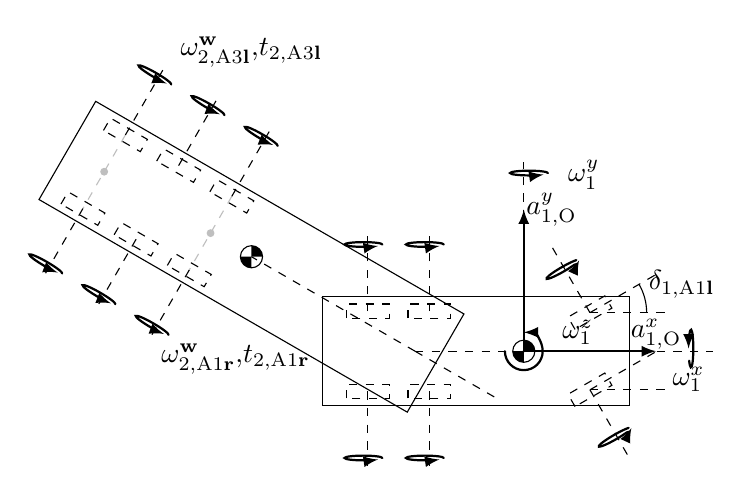
\begin{tikzpicture}
    \def\scale{0.6}
    % Tractor Dimensions
    \def\lTract{6.5*\scale}
    \def\wTract{2.3*\scale}
    \def\firstAxleTract{-\lTract+0.5}*\scale
    \def\lCoup{3.7*\scale}
    \def\cogxOne{-1.4*\scale}

    \def\trackWidthTract{(\wTract/2-0.3*\scale)}

    % Trailer Dimensions
    \def\lTrail{9*\scale}
    \def\wTrail{2.4*\scale}
    \def\cogxTwo{4*\scale}
    \def\lFrontTrail{0.5*\scale}
    \def\lAxleTrailCoupling{5*\scale}

    \def\trackWidthTrail{(\wTrail/2-0.3*\scale)}

    % Axle Distances
    \def\AxDistOne{3.4*\scale}
     \def\AxDist{1.3*\scale}

    % Tyre Dimensions
     \def\lTire{0.9*\scale}
     \def\wTire{0.3*\scale}

     \def\nodeDist{0.3*\scale}

     
     % Angles
    \def\ang{-30}
    
     \def\sAngL{30}
     \def\sAngR{30}

    % Calculations
    \def\lTrailRecX{-cos(\ang)*(\lCoup)+\lFrontTrail}
    \def\ArcSize{2*\scale}
    
    \def\lTrailRecY{sin(\ang)*(\lCoup)-\wTrail/2}
     \def\trailCOGX{-\lCoup-cos(\ang)*(\cogxTwo)}
     \def\trailCOGY{-sin(\ang)*(\cogxTwo)}

     
     \coordinate (CoG1) at (\cogxOne,0);
     \coordinate (Coup) at (-\lCoup,0);
     \coordinate (Coup2) at (-\lCoup+\ArcSize,0);
     \coordinate (Coup3) at ({-\lCoup+cos(\ang)*\ArcSize},{sin(\ang)*\ArcSize});
     \coordinate (rearTrail) at ({\trailCOGX},{\trailCOGY});

     \def\tireLeftX{}
     \def\tireRight{-sin(\sAng)*(2)}

    % Trailer Tires, needs to be rotated to match the angle of the trailer.
    % As the coupling point is at almost the rear of the tractor, we need to offset the tires by the distance of the coupling point.
    % and then the rotated length to the first axle of the trailer. We also need to add the "sine of length" to the y coordinate.
    \coordinate (firstAxle) at ({-\lCoup-cos(\ang)*(\lAxleTrailCoupling)}, {-sin(\ang)*(\lAxleTrailCoupling)});
    \coordinate (thirdAxle) at ({-\lCoup-cos(\ang)*(\lAxleTrailCoupling+\AxDist*2)}, {-sin(\ang)*(\lAxleTrailCoupling+\AxDist*2)});
    \coordinate (CoG2) at ({\trailCOGX}, {\trailCOGY});



    %% Some additional lines
    % Calculate the left and right tire positions of the firstAxle, needs to be rotated to match the angle of the trailer.
    \coordinate (tireLeft) at ($(firstAxle) + ({-sin(\ang)*\trackWidthTrail)},{cos(\ang)*\trackWidthTrail})$);
    \coordinate (tireRight) at ($(firstAxle) - ({-sin(\ang)*\trackWidthTrail},{cos(\ang)*\trackWidthTrail})$);

    % Draw a dashed line between tireLeft and tireRight
    \draw[dashed] (tireLeft) -- (tireRight);

    % Calculate the left and right tire positions of the firstAxle, needs to be rotated to match the angle of the trailer.
    \coordinate (tireLeft3) at ($(thirdAxle) + ({-sin(\ang)*\trackWidthTrail},{cos(\ang)*\trackWidthTrail})$);
    \coordinate (tireRight3) at ($(thirdAxle) - ({-sin(\ang)*\trackWidthTrail},{cos(\ang)*\trackWidthTrail})$);

    % Draw a dashed line between tireLeft and tireRight
    \draw[dashed] (tireLeft3) -- (tireRight3);

    % Add a marker for the center of these axles
    \fill[black] (firstAxle) circle (0.05);
    \fill[black] (thirdAxle) circle (0.05);

    % Main Bodies
    \fill[nearly opaque,white,rotate=\ang] ({\lTrailRecX},{\lTrailRecY}) rectangle++ (-\lTrail,\wTrail) node[midway] {};
    \fill[nearly opaque,white] (\firstAxleTract,-\wTract/2) rectangle++ (\lTract,\wTract) node[midway] {};
    \draw[] (\firstAxleTract,-\wTract/2) rectangle++ (\lTract,\wTract) node[midway] {};
    \draw[,rotate=\ang] ({\lTrailRecX},{\lTrailRecY}) rectangle++ (-\lTrail,\wTrail) node[midway] {};
    % Notes
    \node at (\cogxOne,0) {$\centerofmass$};
    \node at ({\trailCOGX},{\trailCOGY}) {$\centerofmass$};

    % Articulation Angle
    \draw[dashed] (Coup) to (Coup2);
    \draw[dashed] (Coup) to (Coup3);
    \draw[dashed] (Coup) to (rearTrail);
    % \draw pic["$\psi_{1/2}^z$",draw=black,angle radius=40*\scale,angle eccentricity=1.8*sqrt(\scale)] {angle=Coup3--Coup--Coup2};   

    % Coupling Force
    % \draw[force] (Coup) --++ (1.2*\scale,0) node[right={\nodeDist},above=\nodeDist] {$f^x_{1,\Cr}$};
    % \draw[force] (Coup) --++ (0,2*\scale) node[right=\nodeDist] {$f^y_{1,\Cr}$};

    % Velocity in CoG
    \draw[force] (CoG1) --++ (2.8*\scale,0) node[above=-0.1] {$a^x_{1,\CG}$};
    \draw[force] (CoG1) --++ (0,3*\scale) node[right={-0.1}] {$a^y_{1,\CG}$};

    \draw[dashed] (CoG1) to (\cogxOne,{4*\scale});
    \draw[force] (\cogxOne,{4.2*\scale}) ++(320:.4) arc[start angle=0, end angle=320, x radius=0.4*\scale,y radius=0.05*\scale] node[right={\nodeDist}] {$\omega^y_{1}$};
    \draw[dashed] (CoG1) to ({\cogxOne+4*\scale},{0});
    \draw[force] ({\cogxOne+3.5*\scale},{-0.2*\scale}) arc[start angle=-140, end angle=180, y radius=0.4*\scale,x radius=0.05*\scale] node[below=0.1] {$\omega^x_{1}$};
    % Yaw Rate, arc centered around CoG, around 270 degrees, for both tractor and trailer
    \draw[force] (CoG1) ++(-0.4*\scale,0) arc (-180:90:0.4*\scale) node[above={\nodeDist}, right=\nodeDist*2] {$\omega^z_{1}$};

    
    % Rotated Tires
    \draw[dashed,rotate around={\sAngL:(0,{(\wTract-0.4)/2})}] (-\lTire/2,{(\wTract-0.4)/2 - \wTire/2}) rectangle++ (\lTire,\wTire) node[midway] {};
    \draw[dashed,rotate around={\sAngR:(0,{-(\wTract-0.4)/2})}] (-\lTire/2,{-(\wTract-0.4)/2 - \wTire/2}) rectangle++ (\lTire,\wTire) node[midway] {};
     
    % Straight Tires
    \foreach \x in {{-\AxDistOne},{-\AxDistOne-\AxDist}}{
    \foreach \y in {-\trackWidthTract,\trackWidthTract}{
        \draw[dashed] ({\x-\lTire/2},{\y - \wTire/2}) rectangle++ (\lTire,\wTire) node[midway] {};
    }}

    \foreach \x in {0,{\AxDist},{\AxDist*2}}{
    \foreach \y in {-\trackWidthTrail,(\trackWidthTrail)}{
            \def\axleCenterX{-\lCoup-cos(\ang)*(\lAxleTrailCoupling+\x)}
            \def\axleCenterY{       -sin(\ang)*(\lAxleTrailCoupling+\x)}
            \draw[dashed,rotate around={\ang:({\axleCenterX},{\axleCenterY})}] 
                ({\axleCenterX-\lTire/2},{\axleCenterY+\y - \wTire/2}) rectangle++ (\lTire,\wTire) node[midway] {};
    }}

    \draw[dashed] ({0},{-(\wTract-0.4)/2}) --++ ({(1)*cos(\sAngR)},{(1)*sin(\sAngR)}) node[right=\nodeDist/2] {};
    \draw[dashed] ({0},{(\wTract-0.4)/2}) --++ ({(1)*cos(\sAngL)},{(1)*sin(\sAngL)}) node[right=\nodeDist/2] {};
    \draw[dashed] ({0},{-(\wTract-0.4)/2}) --++ (1,0) node[right=\nodeDist/2] {};
    \draw[dashed] ({0},{(\wTract-0.4)/2}) --++ (1,0) node[right=\nodeDist/2] {};

    
    \draw[black] ({0},{(\wTract-0.4)/2}) ++(360:{1.2*\scale}) arc (0:30:1.2*\scale) node[below=4, right=0] {$\delta_{1,\A 1\mathbf{l}}$};
    
     %\sAngR
    \draw[dashed] ({0},{-(\wTract-0.4)/2}) --++ ({-(-1)*sin(\sAngR)},{(-1)*cos(\sAngR)}) node[right=\nodeDist/2] {};
    \draw[dashed] ({0},{(\wTract-0.4)/2}) --++ ({-(1)*sin(\sAngL)},{(1)*cos(\sAngL)}) node[right=\nodeDist/2] {};
    

    \draw[force,rotate around={\sAngR:({0},{-(\wTract-0.4)/2})}] ({0},-1) ++(320:{.4*\scale}) arc[start angle={\sAngR}, end angle={320+\sAngR}, x radius=0.4*\scale,y radius=0.05*\scale] node[above={\nodeDist}, right=\nodeDist] {};
    \draw[force,rotate around={\sAngL:({0},{ (\wTract-0.4)/2})}] ({0}, 1) ++(-320:{.4*\scale}) arc[start angle={\sAngL}, end angle={320+\sAngL}, x radius=0.4*\scale,y radius=0.05*\scale] node[above={\nodeDist}, right=\nodeDist] {};

    
    \foreach \x in {{-\AxDistOne},{-\AxDistOne-\AxDist}}{
    
        \draw[dashed] ({\x},{\trackWidthTract}) to ({\x+0},{\trackWidthTract+1});
        \draw[dashed] ({\x},{-\trackWidthTract}) to ({\x+0},{-\trackWidthTract-1});
        \draw[force] ({\x},{\trackWidthTract+1}) ++(320:{.4*\scale}) arc[start angle=0, end angle=320, x radius=0.4*\scale,y radius=0.05*\scale] node[above={\nodeDist}, right=\nodeDist] {};
        \draw[force] ({\x},{-\trackWidthTract-1}) ++(-320:{.4*\scale}) arc[start angle=0, end angle=320, x radius=0.4*\scale,y radius=0.05*\scale] node[above={\nodeDist}, right=\nodeDist] {};
        }
    %\node[] at ({-\AxDistOne-\AxDist+0.7}, 1.6) {$\omega^\mathbf{w}_{1,\A 3\mathbf{l}}$,$t_{1,\A 3\mathbf{r}}$};
    \foreach \x in {0,{\AxDist},{\AxDist*2}}{
            \def\axleCenterX{-\lCoup-cos(\ang)*(\lAxleTrailCoupling+\x)}
            \def\axleCenterY{       -sin(\ang)*(\lAxleTrailCoupling+\x)}

            \draw[dashed,rotate around={\ang:({\axleCenterX},{\axleCenterY})}] ({\axleCenterX},{\axleCenterY+\trackWidthTrail}) --++ ({0},{1});
            \draw[dashed,rotate around={\ang:({\axleCenterX},{\axleCenterY})}] ({\axleCenterX},{\axleCenterY-\trackWidthTrail}) --++ ({0},{-1});
           % \draw[force,rotate around={\ang:({\axleCenterX},{\axleCenterY})}] ({\axleCenterX},{\axleCenterY+\y}) --++ ({1},{0}) node[right=\nodeDist/2] {};
               % Draw arcs around the end of the dashed lines
               
            % Draw arcs around the end of the dashed lines
            \draw[force,rotate around={\ang:({\axleCenterX},{\axleCenterY})}] 
                ({\axleCenterX},{\axleCenterY+\trackWidthTrail+1}) ++(320:{.4*\scale}) arc[start angle=0, end angle=320, x radius=0.4*\scale,y radius=0.05*\scale] node[above={\nodeDist}, right=\nodeDist] {};
            \draw[force,rotate around={\ang:({\axleCenterX},{\axleCenterY})}] 
                ({\axleCenterX},{\axleCenterY-\trackWidthTrail-1}) ++(-320:{.4*\scale}) arc[start angle=0, end angle=320, x radius=0.4*\scale,y radius=0.05*\scale] node[above={\nodeDist}, right=\nodeDist] {};
            }
    \node[] at ({-4.3}, 3.8) {$\omega^\mathbf{w}_{2,\A 3\mathbf{l}}$,$t_{2,\A 3\mathbf{l}}$};
    \node[] at ({-4.5}, -0.1) {$\omega^\mathbf{w}_{2,\A 1\mathbf{r}}$,$t_{2,\A 1\mathbf{r}}$};
\end{tikzpicture}
    \caption{Available sensor observations, depicting examples of wheel angular velocities and torque. All IMU observations are included except for vertical acceleration $a^z_{1,\CG}$. The steering angle of the left wheel on the first axle is also depicted.}
    \label{fig:measrsmenrts}
\end{figure}

\subsection{Vehicle Parameter Variability and Uncertainty} \label{subsec:vehic_variation}
Accurate knowledge of a vehicle's physical properties is essential for reliable state estimation. While some properties can be precisely determined, others involve uncertainty. Rigid geometric properties, such as axle spacing, coupling point position, and track width, are assumed to be known precisely. However, the longitudinal distance between the first axle $\A 1$ and the CoG of each unit is subject to uncertainty, and treated as such, whereas the vertical distance is assumed unknown. Mass and moment of inertia are treated in the same manner. The nominal tire radii are assumed to be known, though dynamic variations remain uncertain. All other properties are considered unknown.

A truck typically has a long lifespan, during which it undergoes significant changes in load, tire conditions, and driving scenarios. Given this variability, the method should be able to handle these changes. One of the primary factors that varies over the tractor’s lifespan is the trailer's weight. The limit for an articulated vehicle is around $40$ tonnes in Europe\cite{noauthor_council_1996}.
Further, the cornering stiffness of a given tire is rarely well-defined, as it varies with factors such as temperature, pressure, and age. However, the distribution of cornering stiffness across all tires can be studied \cite{hjort_tyre_2021}. For this study, we assume the distribution is known.

% If I have time to regenerate the simulations, I want a mixture of a normal and uniform distribution.

%%%%%%%%%%%%%%%%%%%%%%%%%%%%%%%%%%%%%%%%%%%%%%%%%%%%%%%%%%%%%%%
%%%% DYNAMIC MODEL
%%%%%%%%%%%%%%%%%%%%%%%%%%%%%%%%%%%%%%%%%%%%%%%%%%%%%%%%%%%%%%%
\section{Decoupled dynamic model}\label{sec:model}
When describing two connected objects with articulation, the resulting dynamic model is a differential algebraic equation (DAE)\cite{ghandriz_computationally_2020} of a high degree. Although this DAE is solvable, it's unfeasible to use in real-time due to its complexity. The primary goal of this work is to derive a model that reduces the complexity, without resorting to a linearized model. This Section derives the time-continuous dynamic model and is split into four subsections.

To simplify the model, we assume the ground is locally planar, constraining both units to the same flat plane. Each unit's body frame remains parallel to the ground, so their relative angular displacement occurs only around the normal direction, $z$. This articulation angle, $\psi^z_{1/2}$, represents the angle from the second to the first unit. This simplification removes suspension dynamics, focusing on primary interactions.

\subsection{Coupling Forces with Damper}\label{subsec:coupForce}
The complexity of the DAE is solved by introducing a damper between the two units, instead of a rigid connection. By this introduction, we can jointly model the essential states, including the coupling forces, articulation angle, and lateral velocity. This approach eliminates the need to consider a shifting center of mass for both units due to articulation angle changes. Instead, we explicitly model the coupling forces, providing a more accurate and stable representation of the vehicle dynamics. In essence, this damper tries to balance the forces of each unit to behave in the same manner. 

The force $f$ acting on a damper is described by $f = -C^d v$, where $C^d$ represents the damper constant and $v$ denotes the relative velocity. 
In this application, the relative velocity is the difference in velocity between the two units, the tractor and the trailer. Specifically, it refers to the velocities at the coupling points, $\bm{v}_{1,\Cr}$ and $\bm{v}_{2,\Cf}$, respectively. Using this model, the coupling force can be expressed as
\begin{align}
    \bm{f}_{1,\Cr}(t) &= -\bm{C}^d_1\odot (\bm{v}_{1,\Cr}(t) - R^{2\times2}(\psi^z_{1/2}(t))\bm{v}_{2,\Cf}(t))\label{eq:main},
\end{align}
where $\bm{C}^d_1 = [C^{dx}_1,C^{dy}_1]^\top$, and $\odot$ being an element wise multiplication.
%$R^{2\times2}(\psi^z_{1/2}(t))$ is the rotation matrix transforming a vector from the frame of unit 2 to unit 1,
$R^{2\times2}$ is the rotation matrix,
\begin{equation}
    R^{2\times2}(\alpha) = \begin{bmatrix}
        \cos\alpha & \sin\alpha \\
        -\sin\alpha & \cos\alpha
    \end{bmatrix}.
\end{equation}
used to describe the second unit's velocities in the first unit's coordinate frame.

To describe the force in terms of the velocities in the center of gravity (CoG) of each unit, $\bm{v}_{i,\CG}$. Using the CoG simplifies the analysis since it represents the point where the system’s mass is concentrated, making it easier to separate translational and rotational motion. We note that velocities in the coupling point can be expressed as,
\begin{align}
    \bm{v}_{i,\text{P}}(t) &= \bm{v}_{i,\CG}(t) + \bm{\omega_i}(t)\times \bm{l}_{i,\Cr/\CG}, \label{eq:v1crcf}
\end{align}
where $\times$ denotes the cross product and $\bm{l}_{i,\Cr/\CG}$ is the distance between the coupling point and CoG for unit $i$. 
Combined with \eqref{eq:main} yields,
\begin{align}
    \bm{{f}}_{1,\Cr}(t) &= -\bm{C}^d_1\odot ({\bm{v}}_{1,\CG}(t)+\bm{\omega}_1(t)\times\bm{l}_{1,\Cr/\CG}-\label{eq:coupForce}
    \\ &R^{2\times2}(\psi^z_{1/2}(t)) ({\bm{v}}_{2,\CG}(t)+\bm{\omega}_2(t)\times\bm{l}_{2,\Cr/\CG})), \nonumber
\end{align}
describing the coupling forces based on available states. 

Finally, the dynamics of the coupling force is found through differentiating \eqref{eq:coupForce} with respect to time. The expression is not detailed here for brevity, but the resulting dynamic model for the coupling forces is summarized as
\begin{equation}\label{eq:forceDiff}
    \dot{\bm{f}}_{1,\Cr}(t) = \frac{d}{dt}\bm{{f}}_{1,\Cr}(t) + \bm{q}^{f_c}(t).
\end{equation}
where $\bm{q}^{f_c}$ is a white noise process added to describe simplifications and modeling errors, we assume that ${{\omega}}^x_1(t)$ and ${{\omega}}^y_1(t)$, are small, i.e., relatively smooth dynamics. Note that the differentiation of \eqref{eq:coupForce} depends on the accelerations, $\dot{\bm{v}}_{i,\CG}(t)$, and change in yaw rate, $\dot{{\omega}}^z_i(t)$, for each unit, which are detailed in Section \ref{subsec:ForceDriven}.

%%%%%%%%%%%%%%%%%%%%%%%%%%%%%%%%%%%%%%%%%%%%%%%%%%%%%%%%%%%%%%%
%%%% FORCE DRIVEN
%%%%%%%%%%%%%%%%%%%%%%%%%%%%%%%%%%%%%%%%%%%%%%%%%%%%%%%%%%%%%%%

\subsection{Force Driven States} \label{subsec:ForceDriven}
This section derives the linear acceleration for each unit, $\dot{\bm{v}}_{1,\CG}(t)$, and $\dot{\bm{v}}_{2,\CG}(t)$ and the change in yaw rate for each unit, $\dot{{\omega}}^z_1(t)$, and $\dot{{\omega}}^z_2(t)$. These states, as the title hints, are obtained using Newton’s Second Law, $f=ma$. The forces acting on the vehicle are from each axle, $\bm{f}_{i,\A 1}(t)$, $\bm{f}_{i,\A 2}(t)$ and $\bm{f}_{i,\A 3}(t)$, forces from the coupling point, $\bm{f}_{i,\Cr}(t)$, and gravitational forces, $\bm{f}_{i,g}(t)$. By denoting the set of these force positions as $\mathcal{L}$, the linear accelerations for unit $i$ are given by
\begin{align}
    \dot{\bm{v}}_{i,\CG}(t) &= \sum_{j\in \mathcal{L}}\bm{f}_{i,j}(t)/m_i - \bm{\omega}_i(t)\times\bm{v}_{i,\CG}(t) + \bm{q}^v(t), \label{eq:vdot} \\
    \dot{\omega}^z_i(t) &= \sum_{j\in \mathcal{L}}\left(\bm{f}_{i,j}(t)^\top \bm{l}_{i,j/\CG} \right) /J_i^z + \bm{q}^{z\omega}(t)\label{eq:omegadot}
\end{align}
where $J^z_i$ is the moment of inertia around the z-axis. %For the linear acceleration, 
The cross product between angular and translational velocity is added to account for the effects of rotating the vehicle's reference frame. Finally, the white noise processes $\bm{q}^v$ and $\bm{q}^{z\omega}$ are added to account for uncertainty and errors in this model.

To express \eqref{eq:vdot} and \eqref{eq:omegadot} we need the the lateral and longitudinal components of the axle forces on unit $i$, denoted as $f^x_{i,\A a}$ and $f^y_{i, \A a}$ for each axle $\A a$ (where $a\in[1 \, .. 3]$). For the lateral component, we use a simple tire model\cite{pacejka_tyre_2006} and assume operation within the linear region,
\begin{equation}
    f^{y}_{i,\A a,s}(t) = f^z_{i,\A a}(t) C^{cc}_{i,\A a} s_{i,\A a,s}(t)
\end{equation}
where $f^z_{i,\A a}$ represents the vertical force, $C^{cc}_{i,\A a}$ is the cornering coefficient of axle $a$ in unit $i$, and $s_{i,\A a,s}(t)$ is the slip angle, with $s$ denotes left or right side.
The slip angle is simply the direction of the vector $\bm{v}_{i,\A a, s}$, and is mathematically expressed as 
\begin{equation}
    s_{i,\A a}(t) = \arctan\frac{v^y_{i,\A a,s}(t)}{|v^x_{i,\A a,s}(t)|}.
\end{equation}
The vertical forces can vary significantly in dynamic situations, but to model them well requires precise knowledge of the CoG height. To simplify the problem, they are assumed static and determined by solving a system of equations. Under the assumption of no acceleration or change in angular velocity, force and moment equilibrium can be expressed for each unit. Additionally assuming $f^z_{1,\A 2} =f^z_{1,\A 3}$ and $f^z_{2,\A 1} =f^z_{2,\A 2} =f^z_{1,\A 3}$, based on the idea that the suspension system distributes these forces, the system takes the form $Ax=b$. Solving this system yields the vertical forces, including the vertical coupling force.

The longitudinal axle forces have two components, one depending on the rolling resistance, $C^{rr}_{i}$, and one on the applied torque, $\tau_{i,\A a, s}(t)$, coming either from the drive line or the brakes. To account for differential braking, the force is expressed for each side $s$ separately
\begin{equation}
    f^x_{i,\A a, s}(t) = f^z_{i,\A a,s}(t)C^{rr}_i + \frac{\tau_{i,\A a,s}(t)}{r_{i,\A a, s}},
\end{equation}
where $r_{i, \A a,s}$ is the corresponding tire radius.

For the steerable axle, the coordinate system must be transformed to compute the tire forces. This is done by rotating the velocities to the vehicle frame as follows:
\begin{align}
    \bm{v}_{w,\A 1,\text{l}} &= R(\delta_{1,\A 1,\text{l}})\bm{v}_{1,\A 1,\text{l}}, \\
    \bm{v}_{w,\A 1,\text{r}} &= R(\delta_{1,\A 1,\text{r}})\bm{v}_{1,\A 1,\text{r}}. 
\end{align}
Similarly, the forces must be expressed in the vehicle frame:
\begin{align}
    \bm{f}_{1,\A 1,\text{l}} &= R(\delta_{1,\A 1,\text{l}})^\top\bm{f}_{w,\A 1,\text{l}}, \\
    \bm{f}_{1,\A 1,\text{r}} &= R(\delta_{1,\A 1,\text{r}})^\top\bm{f}_{w,\A 1,\text{r}}.
\end{align}

The gravitational force is assumed to be constant but acts in different directions depending on the alignment between each unit's frame and the world frame, requiring appropriate rotation
\begin{align}
    \bm{f}_{i,g}(t) &= R_{i/\w}(t)[0,0,-g]^\top.  \label{eq:gravForce}
\end{align}
Here, $R_{i/\w}$ is the rotation matrix that expresses how vectors from the world frame appear in unit $i$’s frame. For the first unit, this transformation is defined by its roll, $\alpha^x_1$, and pitch, $\alpha^y_1$, angles relative to the world frame:
\begin{align}
    R_{1/\w}(t) = (R_x(\alpha^x_{1/\w}(t)) R_y(\alpha^y_{1/\w}(t)))^\top.
\end{align}
Note that the unit's yaw angle does not affect the gravitational force and is therefore excluded.
For the second unit, the rotation matrix $R_{2/\w}$ is determined based on the articulation angle and the rotation matrix of the first unit. Since the articulation angle $\psi^z_{1/2}$ represents the rotation about the vehicle's z-axis from trailer to tractor and is applied last, the resulting transformation is given by
\begin{align}
    R_{2/\w}(t) = R_z(\psi^z_{1/2}(t)) R_{1/\w}(t).
\end{align}

%%%%%%%%%%%%%%%% POSE %%%%%%%%%%%%%%%
\subsection{Pose} \label{subsec:pose}
The pose of the vehicle combination concerns how the units are aligned in the world. The states of interest are the roll $\alpha^x_1$, and pitch $\alpha^y_1$ angles of the first unit relative to the world frame, as well as the articulation angle $\psi^z_{1/2}$ between the units.
The dynamics of the articulation angle are modeled as
\begin{equation}
    \dot{\alpha}^z_{1/2}(t) = \omega^z_1(t) - \omega^z_2(t) + q^{\alpha,z}(t) \label{eq:artAngle}
\end{equation}
where $q^{\alpha,z}(t)$ is a known white noise process introduced to account for misalignments caused by assuming that the units are aligned with the tractor's $z$-axis.

The time derivatives of the pitch and roll angles can be expressed in terms of the body-fixed angular velocities $\bm{\omega}_1(t)$ through the Euler Angle Rate Transformation\cite{hover_system_2021}
\begin{align}
    \dot{\bm\alpha}_1 =
    \begin{bmatrix}\dot{\alpha}^x_1(t) \\ 
    \dot{\alpha}^y_1(t) \end{bmatrix} =
\bm{J}(t) \bm{\omega}_1(t), \label{eq:euler}
\end{align}
where
\begin{equation}
    \bm{J}(t) = \begin{bmatrix}
1 & \sin\alpha^x_1(t) \tan\alpha^y_1(t) & \cos\alpha^x_1(t) \tan\alpha^y_1(t) \\
0 & \cos\alpha^x_1(t) & -\sin\alpha^x_1(t)
\end{bmatrix}.
\end{equation}
Since these are direct transformations, no uncertainty is added.

To complete the model, we need to model the dynamics of the body-frame roll and pitch rates, $\dot \omega^x_1$ and $\dot \omega^y_1$. Assuming the vehicle is parallel to the ground, these are driven by changes in the road condition. As we assume no explicit knowledge of the road, the rates are modeled as,
\begin{align}
    \dot{\omega}^x_1(t) &= q^{x\omega}(t), \label{eq:omegaDotx}\\
    \dot{\omega}^y_1(t) &= q^{y\omega}(t). \label{eq:omegaDoty}
\end{align}
where $q^{x\omega}$ and $q^{y\omega}$ are known white noise processes. 

\subsection{Complete Model} \label{subsec:params}
In sum, the final process model is formed from \eqref{eq:vdot}, \eqref{eq:omegadot}, \eqref{eq:omegaDotx}, \eqref{eq:omegaDoty}, \eqref{eq:artAngle}, \eqref{eq:euler}, and \eqref{eq:forceDiff} and combined into
\begin{equation}
    \dot{\bm{x}}(t) = \bm{G}(\bm{x}(t),\bm{u}(t), \bm{\theta}) + \bm{q}(t), \label{eq:contModel}
\end{equation}
where
\begin{align}
    \bm{x}(t) &= [v^x_{1,\CG}(t),v^y_{1,\CG}(t),
        \omega^x_1(t),
        \omega^y_1(t),
        \omega^z_1(t),
        \omega^z_2(t),\nonumber \\&
        \psi^z_{1/2}(t),
        \alpha^x_1(t), 
        \alpha^y_1(t),
        f^x_{1,\Cr}(t),
        f^y_{1,\Cr}(t)]^\top,\label{eq:states}\\
    \bm{u}(t) &= [\bm\tau_1(t),\bm\tau_2(t),\delta(t)]^\top,
\end{align}
and $\bm{q}(t)$ is a vector with corresponding noise processes.
The parameter vector  
\begin{align}
\bm{\theta}= &[m_1,m_2,l^x_{1,\CG/\A 1},J^z_1,J^z_2,l^x_{2,\CG/\A 1},r_{1,l},r_{1,r},r_{2,l},r_{2,r}, \nonumber \\ 
&C^{cc}_{1,\A 1},C^{cc}_{1,\A 2},C^{cc}_{1,\A 3},C^{cc}_{2,\A 1},C^{cc}_{2,\A 2},C^{cc}_{2,\A 3}, \nonumber \\
&{C}^{dx}_1,{C}^{dy}_1,C^{rr}_1,C^{rr}_2]^T.
\end{align}
contains the constant but uncertain parameters introduced in Section \ref{sec:model}.

%%%%%%%%%%%%%%%%%%%%%%%%%%%%%%%%%%%%%%%%%%%%%%%%%%%%%%%%%%%%%%%
%%%% FILTER
%%%%%%%%%%%%%%%%%%%%%%%%%%%%%%%%%%%%%%%%%%%%%%%%%%%%%%%%%%%%%%%
\section{Filter}\label{sec:filter}
To estimate the state vector given noisy sensor measurements, we employ an Unscented Kalman Filter (UKF) as a Bayesian estimator to recursively approximate the posterior state distribution in \eqref{eq:posterior} based on the proposed model. The UKF is well-suited for handling model nonlinearities and provides a structured approach to accounting for parameter uncertainties. This section describes the process model, the formulation of measurement equations, and the treatment of these parameter uncertainties.

\subsection{Process Model}
The process model requires a discrete-time representation to predict the state at the next time step. Presented model \eqref{eq:contModel} is however continuous and must be discretized. This is achieved using the Euler approximation
\begin{align}
    \bm{x}(T(k+1)) &\approx \bm{x}(Tk) + \\\nonumber &T\bm{G}(\bm{x}(Tk), \bm{u}(Tk), \bm{\theta}) + T\bm{q}(Tk), 
\end{align}
where $k$ is discrete-time index and $T$ is the sampling interval. The Euler approximation is chosen for its computational efficiency and the small sampling interval. During testing, no significant system delays were observed.

\subsection{Measurement Model}
The filter relies on sensor measurements that are inherently noisy and based on modeling assumptions. Below we define the measurement equations for acceleration, angular velocity, and wheel angular velocity.
\begin{equation}
    \bm{z}[k] = \bm{H}({\bm{x}}[k],\bm{u}[k],\bm{\theta}),    
\end{equation}
where the vector ${\bm{z}}[k] = [{\hat{\bm\omega}}^w_1,\hat{\bm\omega}^w_2,\hat{\bm{a}}_1,\hat{\bm\omega}_1]$.
The following subsection covers how each sensor is modeled in the vector $H$. Note that while $\bm{\theta}$ appears in $\bm{H}$, only a subset is relevant to the measurement model. 
\subsubsection{Acceleration}
The experienced acceleration, denoted $\bm{a}$, differs from the linear acceleration defined in \eqref{eq:vdot} because $\bm{a}_{i,\CG}(t)$ excludes gravitational acceleration and the additional effects arising from the changing body-fixed reference frame. It is therefore given by
\begin{equation}
    \bm{a}_{i,\CG}(t) = \left(\sum_{j \in \mathcal{L}\setminus g}\bm{f}_{i,j}(t)\right)/m_i,  \label{eq:acc}
\end{equation}
where the summation includes all non-gravitational forces acting on unit $i$. As discussed in Section \ref{subsec:sensors}, the bias in the acceleration measurement is assumed to be small or compensated by the sensor. As such, we model the accelerometer measurement at time $k$ as
\begin{equation}
    \hat{\bm{a}}_{1,\A 1}[k] = \bm{a}_{1,\A 1}[k] + \bm{w}^{a}[k],
\end{equation}
where $\bm{a}_{1,\A 1}$ is defined in \eqref{eq:acc} and $\bm{w}^{a}$ is a white zero-mean Gaussian noise process with known covariance.

\subsubsection{Angular Velocity}
Similarly, the angular velocity measurements are assumed unbiased and, thus, modeled as 
\begin{equation} \hat{\bm{\omega}}_1[k] = \bm{\omega}_1[k] + \bm{w}^{\omega}[k] \end{equation} 
where $\bm{w}^{\omega}$ is white zero-mean Gaussian measurement noise with known covariance. 

\subsubsection{Wheel Angular Velocity}
Let $\omega^w_{i,\A a,s}$ denote the angular velocity of the wheel on unit $i$, axle $a$, and side $s$. Assuming negligible longitudinal slip and a constant tire radius, the angular velocity is modeled as
\begin{equation}
    \hat{\omega}_{\t i,\A a,s}[k] = v^{x}_{i,\A a,s}/r_{i,\A a,s} + w^{\omega}_{\t i,\A a,s}.
\end{equation}
Here the white noise $w^{\omega}_{\t i,\A a,s}$ represents the error introduced by the assumptions.

\subsection{Uncertainty of Parameters}\label{subsec:uncertainty}
Both the motion and measurement model depend on a set of unknown but important parameters, $\bm{\theta}$. To allow the filter to accurately reflect the uncertainty in the predicted state and measurement, we select sigma points representing an augmented state containing both $\bm{x}$ and $\bm{\theta}$. Using these extended points during runtime allows us to know how parameter uncertainties impact the final estimate.

\section{Evaluation}\label{method}
This section outlines the evaluation process, and the selected test scenarios. Ideally, real-world data would be used, however, obtaining such data presents challenges. This is especially true for measuring the true coupling force, varying the trailer load and changing the cornering stiffness, yet they are key aspects in evaluating coupling force estimation. To overcome this, the model is evaluated using data from a high-fidelity simulation. Measurements are extracted from the simulation's true states and combined with noise before being used in the estimator. The output of the estimator is then compared to the true states of the simulation. The simulation is based on the Volvo Transport Model (VTM), an internal simulator used by Volvo GTT and showcased in a MathWorks seminar \cite{frojd_handling_2021}. VTM has been adapted to meet the needs of this paper.

\subsection{Simulation}\label{method_sit}
A testing framework was implemented where each scenario was simulated at 10 distinct intensity levels, each repeated 10 times for statistical significance. Vehicle parameters were systematically varied to assess the estimator’s robustness. The three scenarios evaluated are as follows.

\parsection{Scenario 1 - Circle}
        The vehicle is driven in a circle at a slowly increasing velocity and constant radius at close to steady-state. Ten radii are tested, linearly distributed between $8-160$m. The lateral acceleration is limited to $0.3$g by limiting the maximum velocity.
        
\parsection{Scenario 2 - Sine-with Dwell}
        The established Sine-with-dwell test sequence adapted for heavy vehicles, described by Laine et al. \cite{laine_proposal_2008}, is commonly used to investigate vehicle performance, albeit on ice. It starts at a set velocity, then releases the throttle and makes a sharp turn left, followed by a sharp turn right. The scenario is run for ten different steering angles, linearly spaced between 1 and 11 degrees, the velocity is adjusted so that the vehicle does not exceed $0.5g$, the length of the turns is also adjusted to change a whole number of lanes.
        
\parsection{Scenario 3 - Incline}
        The vehicle is driven up a hill in varying inclinations, ranging from $\pm10\%$. A velocity is sampled from a uniform distribution between 10 and 25 m/s and held constant throughout. The vehicle is driven in a straight line. This line is at an angle to the steepest incline, thereby creating a banked road, the angle is uniformly sampled between $-2^\circ$ and $2^\circ$. 
 % 
\subsection{Simulation Variations}
To not exceed the maximum load of 40 tonnes, the trailer’s load is uniformly randomized between 0 and 25,000 kg. The load is assumed to have a uniform density, but its placement on the trailer varies. The center of mass is displaced in the longitudinal direction from its default position by $\mathcal{N}(0,0.1)$.

The simulation describes each tire by the magic formula\cite{pacejka_tyre_2006}. The cornering stiffness for each axle is sampled individually for each simulation. This assumes that tires are swapped per axle and experience similar degradation. The distribution is chosen as 
\begin{equation}
    C_{i,\A a} \sim \mathcal{N}(9,1)  \; \forall \; i,a,   \label{Corneringdist}
\end{equation}
to match experimental data\cite{hjort_tyre_2021}.
 
\subsection{Sensor Modeling and Measurement Noise}
IMU signals are generated from the true signals, incorporating noise modeled using the Allan variance of a known sensor\cite{hussen_low-cost_2015}. The IMU is placed in the vehicle's chassis, meaning it is not aligned with the world frame and is affected by both road angle and road to chassis angle. The IMU, located at the first axle, measures
\begin{align}
    \tilde{\bm{a}}_{i,\A 1}[k] &=\bm{a}_{i,\A 1}[k] + \bm{w}^{{a}}_{1,\A 1}[k], \\
    \tilde{\bm{\omega}}_{i}[k] &=\bm{\omega}_{i}[k] + \bm{w}^{{\omega}}_{1,\A 1}[k].
\end{align}
Here, $w^a$ and $w^\omega$ represent additive noise components modeled based on sensor characteristics.

For the wheel angular velocity and steering angle measurements, the problem formulation suggests that noise is minimal and does not significantly affect the results
\begin{align}
    \tilde{\bm{\omega}}_{\text{t} i,\A a, s} &= \bm{\omega}_{\text{t} i,\A a, s}, \\
    \tilde{\bm{\delta}}_{\text{t} i,\A a, s} &= \bm{\delta}_{\text{t} i,\A a, s}.
\end{align}

Drive and brake torque measurements, $\bm{\tau}_i$ serve as inputs to both estimator and simulation. However, the simulation includes detailed and accurate modeling of losses in the driveshafts, tires, axles, and other components, which are not known to the estimator. This means that while the simulation accounts for these losses, the estimator operates without this detailed information. Although the exact nature of these losses is complex and not easily presented, they can be recreated using the simulator. The effects of these losses are inherently present in the simulation data, reflecting the real-world complexities of torque transmission through the vehicle's drivetrain.

\subsection{Filter and Model Parameters}
This section goes over the parameters used in the filter and the model, tuned on a calibration set, smaller and distinct from the test set. Each $q$ is scaled by the sampling time $T$ and are as follows, $\bm{q}^v\sim\mathcal{N}(\bm0,\operatorname{diag}(0.001,0.01))$, $\bm{q}^{z\omega}\sim\mathcal{N}(\bm0,\operatorname{diag}(1.7\cdot10^{-4},1.7\cdot10^{-4}))$, ${q}^{\alpha z}\sim\mathcal{N}(0,1.5\ex{-5})$, finally $q^{x\omega}\sim\mathcal{N}(0,10^{-5})$ and $q^{y\omega}\sim\mathcal{N}(0,10^{-5})$. The measurement noises are $\bm{w}^{\omega}\sim\mathcal{N}(0,1\cdot10^{-3}\bm{I})$, $\bm{w}^{a} \sim\mathcal{N}(0,0.3\bm{I})$, where $\bm{I}$ is the appropriate identity matrix. Further, each $w^{\omega w}_{i,\A a, s}\sim\mathcal{N}(0,8.9\ex{-3})$. Initial uncertainties were set high to demonstrate convergence. In the same order as \eqref{eq:states}, $P[0]$ is initialized as a diagonal matrix with entries $10^{k_i}$, where $\bm{k} = -[2,2,5,5,5,5,3,4,4,0,0]$.

Model parameters are based on knowledge of the vehicle, according to \ref{subsec:vehic_variation}. The unknown parameters are $C^{cc}_{i,\A a}\sim\mathcal{N}(9,1) \; \forall \; i,a$, and $r_{i,\A a, s}~=~\bar{r}_{i,\A a} + r^u_{i,s}$, where $r^u_{i,s}\sim\mathcal{N}(0,0.02) \; \forall \; i, s$. Finally $C^{rr}_i\sim\mathcal{N}(0.01,0.002) \; \forall \; i$. $\bm{C}^d$ does not have a real-life physical counterpart, but its value is here motivated by the damping ratio, $\zeta$, which characterizes the frequency response and is defined as the actual damping divided by critical damping, $c_c~=~2\sqrt{C^km}$. $C^k$ is the spring constant and not defined for this system. By this motivation the constants are tuned to $C^{dx}=0.5\sqrt{m_1+m_2}$, $C^{dy}=0.2\sqrt{m_1+m_2}$ to maintain similar response over different loads.

\subsection{Performance Metric}\label{method_eval}
We evaluate three key metrics, Root Mean Square Error (RMSE), Average Normalized Estimation Error Squared (ANEES)\cite{chen_weak_2018}, and max error. As each state component varies significantly in scale, we evaluate each component separately. 

The UKF approximates the posterior distribution, as a Gaussian, with mean, $\hat{\bm{x}}[k]$, and covariance, $\bm{P}[k]$. The error, $\epsilon_j[k]$, is calculated from this mean, and the simulated true value, $x_j[k]$, at each time step,
\begin{equation}
    \epsilon_j[k] = \hat{x}_j[k] - x_j[k].
\end{equation}
The RMSE and ANEES are averaged over experiments, while the maximum error is the largest observed. The metrics for each experiment are calculated accordingly,
\begin{align}
    RMSE_j &= \sqrt{\frac{1}{\text{N}}\left(\sum_k (\epsilon_j[k])^2\right)}, \\
    ANEES_j &= \frac{1}{\text{N}}\sum_k\epsilon_j[k]P_{j,j}[k]^{-1}\epsilon_j[k], \\
    \text{Max }\epsilon_j &= \max_{k}|\bm{\epsilon}_j[k]|
\end{align}
here, N is the total number of steps in an experiment. ANEES quantifies how well the estimator can express its uncertainty, where a value of 1 is optimal while a larger value indicates over confidence and a lower value means under confidence. In safety related applications, over confidence is typically worse than under confidence.


% \subsection{Baseline}
% The baseline is constructed by describing the entire vehicle without the damper. The remaining force when subtracting acceleration of the trailer from its forces, is the coupling force. As such we can describe the acceleration of the first unit as
% \begin{align}
%     \dot{\bm{v}}_{1,\CG}(t) = &\left(\sum_{j\in \mathcal{L}}\bm{f}_{1,j}(t)- R_z(-\psi^z_{1/2}(t))\sum_{j\in \mathcal{L}}\bm{f}_{2,j}(t) -\bm{a}_2(t)m_2\right)/m_1- \nonumber \\ 
%     &\bm{\omega}_i(t)\times\bm{v}_{i,\CG}(t) + \bm{q}^v(t)
% \end{align}
% where $\bm{a}_2$ is the acceleration of the second unit, 
% \begin{align}
%     \bm{a}_2(t) &= \dot{\bm{v}}_{2,\CG}(t)- \omega_2(t)\times\bm{v}_2 -R_{2/W}\bm{g} \\
%     \bm{v}_{2,\CG} &= \bm{v}_{2,\Cf} - \bm{\omega}_2\times \bm{l}_{\CG/\Cr}, \\
%     \bm{v}_{2,\Cr} &= \bm{R}_z(\psi^z_{1/2})\bm{v}_{1,\Cr}
% \end{align}
% We can express $\dot{\bm{v}}_{2,\CG}(t)$ in terms of our variables and then $\frac{d\bm{v}_2(t)}{dt}$.

%%%%%%%%%%%%%%%%%%%%%%%%%%%%%%%%%%%%%%%%%%%%%%%%%%%%%%%%%%%%%%%
%%%% RESULTS
%%%%%%%%%%%%%%%%%%%%%%%%%%%%%%%%%%%%%%%%%%%%%%%%%%%%%%%%%%%%%%%
\section{Results \& Analysis}
% Börja om med en plan och struktur
% Separera tabell och grafer, börja prata om RMSE kanske
% Ha en tanke med var jag vill presentera, och vilken ordning
% Vore bra att ha resultat utan fjäder som jämförelse
% Overview
This section presents the performance evaluation of the system across various scenarios, based on the defined performance metrics. Table \ref{tab:result} presents the performance of each quantity across different scenarios, using our defined performance metrics. Overall, the RMSE behaves as expected, with lateral coupling force being the most challenging to estimate. The ANEES values are mostly close to 1, with a notable exception in the articulation angle during the circle scenario.
% Highlight some key points in table latvel, latforce (sine), 
Focusing on lateral velocity, the RMSE remains within a few cm/s. Prior studies \cite{ding_event-triggered_2022,villano_cross-combined_2021} report estimators with lateral velocity errors as low as $0.01$m/s on average, with maximum errors up to $0.08$m/s at $65$ km/h, which is consistent with our findings. Direct comparison is limited, however, as these studies focus on cars without trailers. For the trailer, the lateral velocity $v^y_{2,\CG}$ error is slightly larger, but still within a comparable range.

Regarding coupling forces, the longitudinal coupling force error is relatively small, with an RMSE of only a few hundred N. In contrast, the lateral coupling force error is more pronounced. This is worth noting, as the coupling force is influenced by both lateral velocity and cornering stiffness, two factors that are notoriously difficult to estimate.

\begin{table}%[h]
\centering  
\begin{tabular}{llrrr}
 & Set & RMSE & ANEES & Max $|\epsilon|$ \\ 
\hline 
\multirow{ 3 }*{ $v^y_{1,\CG}$ ($m/s$)} 
& circle & $0.017$ & $0.725$ & $0.122$ \\
& sine & $0.010$ & $0.354$ & $0.083$ \\
& slope & $0.009$ & $0.133$ & $0.049$ \\
\cline{2-5} 
\multirow{ 3 }*{ $v^y_{2,\CG}$ ($m/s$)} 
& circle & $0.030$ & $1.154$ & $0.148$ \\
& sine  & $0.014$ & $0.293$ & $0.127$ \\
& slope & $0.008$ & $0.033$ & $0.041$ \\
\cline{2-5} 
\multirow{ 3 }*{ $f^x_{1,\Cr}$ ($kN$)} 
& circle & $0.168$ & $0.351$ & $0.885$ \\
& sine & $0.233$ & $0.860$ & $1.486$ \\
& slope & $0.420$ & $2.195$ & $2.278$ \\
\cline{2-5} 
\multirow{ 3 }*{ $f^y_{1,\Cr}$ ($kN$)} 
& circle & $1.021$ & $1.218$ & $6.782$ \\
& sine & $0.889$ & $1.194$ & $5.559$ \\
& slope & $0.321$ & $0.118$ & $1.842$ \\
\cline{2-5} 
\multirow{ 3 }*{ $\psi^z_{1/2}$ ($^\circ$)} 
& circle & $0.314$ & $2.796$ & $1.197$ \\
& sine & $0.118$ & $0.443$ & $1.038$ \\
& slope & $0.057$ & $0.132$ & $0.218$
\end{tabular} 
\caption{Estimator performance evaluated on simulated data divided into each scenario for each of the essential states.}
\label{tab:result}  
\end{table} 

To study the typical behavior of our proposed filter, we illustrate three simulation sequences, one per scenario, selected to highlight the strengths and weaknesses of the model.
The circle and sine maneuvers are illustrated in Fig. \ref{fig:circleArt} and Fig. \ref{fig:latSineForce}. While the results are promising and mostly accurate, these reveal that the full dynamics of the vehicle are not entirely captured. Particularly when transitioning back to straight-line driving in the sine maneuver. This limitation is evident in both the coupling force and lateral velocity. One possible explanation for this discrepancy could be the omission of lateral weight transfer, which may play a significant role in these dynamics. This could also explain the offset in articulation angle observed in the circle scenario, as well as the maximum error of $1^\circ$ shown in Tab. \ref{tab:result}.
\begin{figure}
    \centering
    \includesvg[]{imgs/circle}\\
    \caption{Circle Scenario with a 26m radius, iteration 2: Lateral coupling force (top) and articulation angle (bottom).}
    \label{fig:circleArt}
\end{figure}
\begin{figure}
    \centering
    \includesvg[]{imgs/sine}\\
    \caption{Sine scenario with $11^\circ$ steering, iteration 7: Lateral force (top), lateral velocity (middle), and articulation angle (bottom).}
    \label{fig:latSineForce}
\end{figure}
In the slope scenario, shown in Fig. \ref{fig:slopeArt}, the overall force is accurately represented, and the pitch angle estimate, despite some noise, precisely reflects the vehicle's dynamics. While the increase in force at the onset of the incline is not fully captured—likely due to the assumption that the tractor and trailer remain in the same plane—this does not significantly impact the overall accuracy.
\begin{figure}
    \centering
    \includesvg[]{imgs/slope}\\
    \caption{Slope scenario with $6^\circ$ uphill, iteration 1: Longitudinal coupling force (top) and pitch angle (bottom) of the tractor.}
    \label{fig:slopeArt}
\end{figure}
% The execution speed of the proposed decoupled model was measured to be 11.3 times real-time, while the model without decoupling was measured at 0.109 times real-time, under identical conditions. 
% Table \ref{tab:performance_comparison} compares the execution performance of the proposed decoupled model against a baseline without decoupling under identical conditions.
% \begin{table}[h]
% \centering
% \begin{tabular}{|l|c|c|}
% \hline
% Metric & Proposal & Baseline \\
% \hline
% Real-Time Execution ($\times$) & $11.5$ & $0.109$ \\
% \hline
% \end{tabular}
% \caption{Comparison of real-time execution performance between the proposal and baseline methods.}
% \label{tab:performance_comparison}
% \end{table}
%%%%%%%%%%%%%%%%%%%%%%%%%%%%%%%%%%%%%%%%%%%%%%%%%%%%%%%%%%%%%%%
%%%% CONCLUSION
%%%%%%%%%%%%%%%%%%%%%%%%%%%%%%%%%%%%%%%%%%%%%%%%%%%%%%%%%%%%%%%
\section{Conclusion}
% Börja om med en plan och struktur
% Vilka claims har vi, vilka experiment/bevis stödjer dem?
The primary contribution of this paper is the development of a novel Bayesian motion estimation framework for articulated heavy vehicles, using a damper-based dynamic model to estimate coupling force, articulation angle, and lateral velocity. By modeling the coupling force as a damper, each unit benefits from the other's information while remaining independently describable. High-fidelity simulations demonstrate the method's robustness across diverse driving conditions, including sensor noise. Inclusion of uncertainty estimates from the Kalman Filter enhances reliability and practical applicability.

Based on the RMSE and maximum error results, we demonstrate that the method provides precise estimates, with lateral velocity RMSE in the range of a few cm/s. While the maximum error in articulation angle is slightly larger than desired, with a deviation of $1^\circ$, this remains a small angle in the context of the overall system. The simplified model effectively captures key dynamics, such as the lateral- and longitudinal coupling forces and pitch angle, though the transition back to straight-line driving in the sine maneuver suggests areas for further refinement.
In conclusion, the proposed model achieves high-precision state estimation even in the presence of sensor noise, validated by competitive error metrics. Although minor deviations exist in lateral force estimation, other states remain unaffected. The Normalized Estimation Error Squared (NEES) metric, used to assess the uncertainty of the estimates, underscores the robustness of the approach. Limitations such as the assumption of planar motion and neglect of lateral weight transfer should be addressed in future work. Broader comparisons to alternative estimation methods and adaptation to low-friction conditions are also important directions, further strengthening the model's applicability to vehicle automation and safety.
\bibliography{references}
\end{document}

